%% This is the main content about this article. I should list them in an order
%% How to balance the existing model, positive and negative instance together, I shall use the dfg-method to create a dfg-matrix to incorporate the impact.
%% how to introduce them into adding long-term dependency feature. After mining the model by Inductive Miner, we have a model without long-term dependency, but we need to change the model and give the right examples.. 
%% If we change the data set, then we need to change the model into another parts, but the current methods can not solve it..
%% Should we also separate them into different sections?? Yes, we need it
%% Also, to delete the silent transition, as one option feature in our methods, we only delete it, in this situation, which will not affect the model behavoirs.

\subsection{Definitions Related To Dfg-Method}
In this part, we provides concepts related to the dfg-method which is based on directly-follows graph. A directly-follows graph as used in \cite{leemans2013discovering}, represents the directly-follows relation of activities in event log. For instance, if there are traces of $\langle ...,A,B,... \rangle$ in event log, one edge (A,B) is added into directly-follows graph. By cutting directly-follows graph under different conditions, Inductive Miner\cite{leemans2013discovering,leemans2014discovering} discovers a process model. Unlike this process, we adapt Inductive Miner to repair model by using existing model, and event log with labels.

\begin{definition}[Cardinality in directly-follows graph]
	Given a directly-follows graph G(L) derived from an event log L, the cardinality of each directly-follows relation in G(L) is defined as:  
	\begin{itemize}
		\item $Cardinality(E(A,B))$ is the frequency of traces with $\langle ...,A,B,... \rangle$. 
		\item Start node A cardinality $Cardinality(Start(A))$ is the frequency of traces with begin node A.
		\item End node B cardinality $Cardinality(End(A))$ is the frequency of traces with end node B.
	\end{itemize}	
\end{definition}
From the positive and negative event log, we can get directly-follows graphs, respectively $G(L_{pos})$ and $G(L_{neg})$. Each edge of  $G(L_{pos})$ and $G(L_{neg})$ has a cardinality to represent the strength of this directly-follows relation. 
However, when the existing model is transformed into  directly-follows graph $G(L_{ext})$, there is no point to assign cardinality on each edge. So we just set 1 to cardinality of each edge. 

%To incorporate all information from  $G(L_pos)$, $G(L_neg)$ and $G(L_ext)$, a data structure is defined directly-follows matrix. 
To incorporate all information from  $G(L_{pos})$, $G(L_{neg})$ and $G(L_{ext})$, we define  weight for each directly-follows relation in graph. 
\begin{definition}[Weight of directly-follows relation]
	Given a directly-follows graph G(L), the weight of each directly-follows relation is defined as \[ Weight(E(A,B)) = \frac{Cardinality(E(A,B))}{Cardinality(E(A,*))}  \] 
	for start activities A, we have 
	\[ Weight(Start(A)) = \frac{Cardinality(Start(A))}{Cardinality(Start(*))} \]
	Similarly for end activities B, we have
	\[ Weight(End(B)) = \frac{Cardinality(End(B))}{Cardinality(End(*))} \]
	E(A,*) means all edges with source A, E(*,B) means all edges with target B, Start(*) represents all start nodes, and End(*) represents all end nodes.
\end{definition}
After defining the weights of each directly-follows relation, for each directly-follows relation, there are three weights from $G_{pos}$, $G_{neg}$ and $G_{ext}$. The following strategy assigns new weight to directly-follows relation to new generated directly-follows graph $G_{new}$.
\begin{definition}[Assign new weights to graph $G_{new}$]
	there are three weights from $G_{pos}$, $G_{neg}$ and $G_{ext}$, the new weight is 
	\begin{itemize}
		\item For one directly-follows relation, \[ Weight(E_{G_{new}}(A,B)) = Weight(E_{G_{pos}}(A,B)) + Weight(E_{G_{ext}}(A,B)) - Weight(E_{G_{neg}}(A,B))\]
		\item For start activities A, we have 
		\[ Weight(Start_{G_{new}}(A)) = Weight(Start_{G_{pos}}(A)) + Weight(Start_{G_{ext}}(A)) - Weight(Start_{G_{neg}}(A)) \]
		\item For end activities B, we have
		\[ Weight(End_{G_{new}}(A)) = Weight(End_{G_{pos}}(A)) + Weight(End_{G_{ext}}(A)) - Weight(End_{G_{neg}}(A)) \]
	\end{itemize}
\end{definition}
After assigning all the weight to directly-follows relation in $G_{new}$, we filter out all directly-follows relation in $G_{new}$ with weight less than 0. 
Then, we transform the $G_{new}$ into process tree bu using Inductive Miner for the next stage.

\subsection{Definitions Related To Add Long-term Dependency}
\textit{Example 1} Consider event log L with labels \[L =[\langle A,C,E \rangle^{50,pos}, \langle B,C,D \rangle^{50,pos}, \langle A,C,D \rangle^{50,neg}]. \] $\langle A,C,E \rangle^{50,pos}$ means there are 10 traces $\langle A,C,E \rangle$ labeled as positive in event log. Similarly, $\langle A,C,D \rangle^{50,neg}$ represents there are $\langle A,C,D \rangle$ traces at number 50 in event log which have negative labels. 

After applying the dfg-algorithm, a model as shown in Figure \ref{fig:pn_without_lt_exm01} is discovered. In event log L, B and D has long-term dependency, and A is expected to support only the execution of E, since $<A,C,D>$ is negative and $<A,C,E>$ is positive. However, the model doesn't express those constraints.
\begin{figure}[h!]
	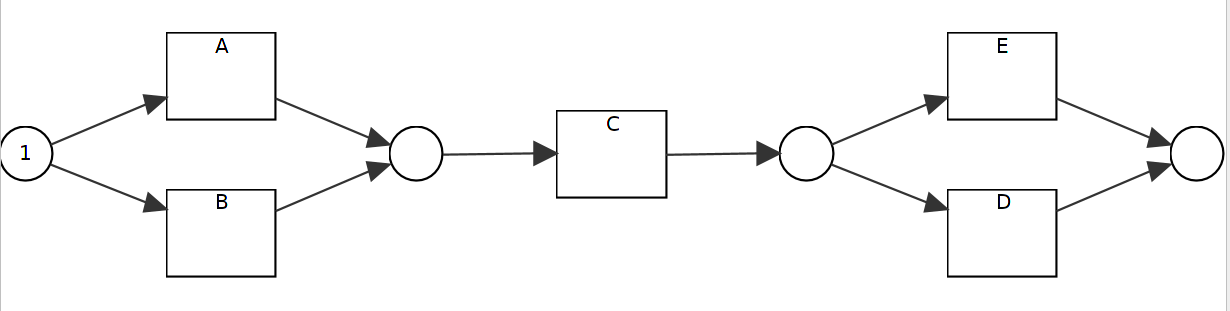
\includegraphics[width=\textwidth]{figures/preliminary/PN06_Seq_2_xor_notnested.png}
	\caption{Process model generated from dfg-algorithm}
	\label{fig:pn_without_lt_exm01}
\end{figure}
Obviously, long-term dependency relates the choices structure in process model, such as exclusive choice, loop and or structure. Due to the complexity of or and loop structure, only the long-term dependency in exclusive choice is considered. 

The inputs for this algorithm are,
\begin{itemize}
	\item Repaired model in process tree
	\item Event log with positive and negative labels
\end{itemize}
The output of this algorithm is: 
\begin{itemize}
	\item Repaired model in petri net with long-term dependency
\end{itemize}
%%if now, we only consider the repaired process tree model, then we don't have problems to make the weights of dfg and long-term dependency unified. But we have it from the existing model, because of existing factor. 
%% Now we have the firstly-repaired model, if we want to create long-term dependency, we also have the 3 weights:: 
%% Ext_Wlt(Si, Tj), but when our negative factor affects, we need to unify them!!To prove it!!! 

Process tree, as one input for the algorithm, is one common model to interpret business process in process mining. It's a block-structured tree. To specify the process tree with respect to long-term dependency, the following definitions are in need. Firstly, the definitions related to tree are reviewed.
\begin{definition}[Tree]
	Let $ \mathscr{E} $ be a finite set of entities, a tree is a collection of entities called nodes, which are connected by edges. A tree T is,
	
	\begin{itemize}
		\item t, with  $t\in \mathscr{E}$, t has no outgoing edges
		\item $t(T_1,T_2,...,T_n)$, with $t\in \mathscr{E}, i,n\in \mathbb{N}, i \leq n ,T_i$ is a tree.
	\end{itemize}
\end{definition}
$T_i$ is a child or subtree of $t(T_1,T_2,...,T_n)$, $t(T_1,T_2,...,T_n)$ is one parent of $T_i$, which can be expressed in $P(t(T_1,T_2,...,T_n),T_i)$. The root of tree is the node without any parent; A tree has only one root. A leaf node is the node which has no children nodes.\\
For a node in a tree, its ancestor and descendant are defined as:
\begin{definition}[Ancestor Relation Anc(A,t)]
	An ancestor of a node t in a tree is a node A, written as $ Anc(A,t) \Rightarrow True$, if those conditions hold,  
	\begin{itemize}
		\item A is a parent of t, written as $ P(A,t) \Rightarrow True$, or
		\item $\exists t_1,t_2..t_n,n\in \mathscr{E}, i < n, P(A,t_1)\land P(t_i,t_{i+1}) \land P(t_n,t) \Rightarrow True $
	\end{itemize}
\end{definition}
The ancestor of root is empty, while leaf nodes has no descendants. Based on this, we define the ancestors set of a node s. 
\begin{definition}[Ancestors of a node a]
	The ancestors set of a node s, Ancestors(s), is defined as: \[ Ancestors(A)=\{t|Anc(t,s) \Rightarrow True \} \]
\end{definition}
Accordingly, descendant relation is given for node t and node s, Des(s,t). If node s is the ancestor of t, then t is a descent of s. $Anc(s,t) \Rightarrow Dec(t,s)$; The set of descendants of node t is Descendants(t).
\begin{definition}[Least Common Ancestor]
	A least common ancestor for node $s$ and node $t$ in a tree is a node n, where 
	\[Anc(n,s) \land Anc(n,t) \land \exists! m Anc(n,m) \land Anc(m,s) \land Anc(m,t) \]
\end{definition}

In process tree, all the leaves are activities in business process, and the middle nodes are operators which represents the relations of all its children nodes\cite{vanderAalst:2016:PMD:2948762,leemans2013discovering}. This paper uses four operators in context of long-term dependency. The four relations.  $\{\rightarrow, \times, \land, \circlearrowright\}$ are considered. 

Next, we only focus on exclusive xor structure on long-term dependency. As known, long-term dependency is associated with choices. In xor block, it means the choices of each xor branch in xor block. For sake of convenience, we define the xor branch.

$Q= \times(Q_1 , Q_2 ,.. Q_n)$, $Q_i$ is one xor branch with respect to Q, rewritten as $XORB_{Q_i}$ to represent one xor branch $Q_i$ in xor block, and record it $XORB_{Q_i} \in XOR_{Q}$. For each branch, there exists the begin and end nodes to represent the beginning and end execution of this branch, which is written respectively as Begin($XORB_{Q_i}$) and End($XORB_{Q_i}$).

%% but the structure of xor branch, do we need to think of right now?? we need to think of it 
For convenience of analysis, two properties of xor block, purity and nestedness are demonstrated to express the different structures of xor block according to its branches.
\begin{definition}[XOR Purity and XOR Nestedness] The xor block purity and nestedness are defined as following: \\
	\begin{itemize}
		\item A xor block $XOR_Q$ is pure if and only $\forall XORB_X \in XOR_Q, XORB_X $ has no xor block descent, which is named as pure xor branch. Else,
		\item A xor block $XOR_Q$ is nested if $ \exists XOR_X, Anc(XOR_Q, XOR_X) \rightarrow True  $. Similarly, this xor branch with xor block is nested.
	\end{itemize}
\end{definition}
%% change the graph for whole explaination!!
In the Figure\ref {fig:xor_nested_branch_variants}, xor block Xor(c1,c2) are pure and not nested, since all the xor branches are leaf node, but xor block Xor(a,Seq(b,Xor(c1,c2))) is impure and nested with Xor(c1,c2). 
\begin{figure}[h!]
	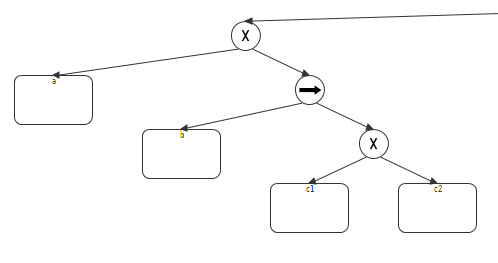
\includegraphics[width=\textwidth]{figures/preliminary/PT02_xor_nested_and_pure.png}
	\caption{XOR branch variants}
	\label{fig:xor_nested_branch_variants}
\end{figure}

%% xor branch, the dependency between them, then how about the dependency on that part, does it exist in the xor block, so we can define it ??
%% the full completeness is also dependency, but sth different, 
%% for arbitrary two xor branches, if they are long-term dependency?? Can I decide, or not ?? I can decide it!! But in the specific way, if they are in a pair, they are ok, else, not !!! 
%% but it goes far, so only write down what I have achieved, but in their thinking way, why in my way?? 
%% given two branch, and they have order, just complexity of implementation, then we only consider the directly ones!!  

Long-term dependency researches on the dependency of choices in xor block, with observation, actually on the pure xor branch, because nested xor branch has multiple choices, which affect the execution of later process. For two arbitrary pure xor branches, to have long-term dependency, they firstly need to satisfy the conditions: (1) they have an order;(2) they have significant correlation.
The order of xor branch follows the same rule of node in process tree which is explained in the following.
\begin{definition}[Order of nodes in process tree]
	Node $X$ is before node $Y$, written in $X \prec Y$, if $X$ is always executed before $Y$.  In the aspect of process tree structure, $X \prec Y$, if the least common ancestor of $X$ and $Y$ is a sequential node, and $X$ positions before $Y$.
\end{definition} 
%% how to define the correlation fo xor branches, if they always happen together
The correlation of xor branches is significant if they always happen together. To define it, several concepts are listed at first. 
\begin{definition}[Xor branch frequency]
	Xor branch $XORB_X$ frequency in event log l is $F_{l}(XORB_X)$, the count of traces with the execution of $XORB_X$. \\
	For multiple xor branches, the frequency in event log l is defined as the count of traces with all the execution of xor branches $XORB_{Xi}$ , written as \[F_{l}(XORB_{X1}, XORB_{X2},...,XORB_{Xn})\].
\end{definition}
%% correlation means the two always happen together, if one not shown, the other also not?? So the connection support.. how to define them?? 
%% connection support, we can say only on number, when it is over one value, 
After calculation of the frequency of the coexistence of multiple xor branches in positive and negative event log, we get the supported connection of those xor branches, and define the correlation. 
\begin{definition}[Correlation of xor branches]
	\label{def: supported-connection}
	For two pure xor branches, $XORB_X \prec XORB_Y$, the supported connection is given as \[SC(XORB_X,XORB_Y)= F_{pos}(XORB_X, XORB_Y) -F_{neg}(XORB_X, XORB_Y)\]. If $SC(XORB_X,XORB_Y) > lt-threshold$, then we say $XORB_X$ and $XORB_Y$ have significant correlation.
\end{definition}

I did some introduction, it is proven that in some cases, we can't deal with it. When the $XORB\_S \neq LT\_S || XORB\_T \neq LT\_T$.

Another way to avoid this problem is to add duplicated events, but the problem stays the same, so if we want to keep the model fit, we add new event for the discovered long-term dependency, the original, we keep it in the model?? But it is not precise!!! It allows too many choices there, but the model is sound, because we add events on model, we produce and consume tokens from duplicated events, and consumes it later.. Still, it is not so right. But if we choose the events before, we decides the events later, it's true... helps a little... 

How to prove it ?? By induction. 
We use  process  trees as one internal result in  our  approach in two factors: (1) they are sound by construction, and can be transferred into sound Petri net models; (2) they are block-structured. which benefits the detection of exclusive relations in model.

\begin{itemize}
	\item the original model is sound
	\item after adding one long-term dependency by duplicating the event, we make sure
	 \\ duplicated events are added into the xor branches, if it's chosen, then it consumes one token, at this xor branches, then it produces two tokens, one of which is put back again into the 
	 To prove the added places and duplicated events between two xor branches will not violate the soundness of model. 
	 \item 
	 \begin{itemize}
	 	\item adding duplicated events of one long-term dependency does not violate the soundness of model. 
	 	
	 	\item To connect the source and target  of long-term dependency which are the duplicated events will not violate the soundness.
	 	\\ One extra place is added to connect the source and target. After executing the source, one token is generated in this place; Due to long-term dependency, only this target is triggered by this token and it consumes this token. No extra token is introduced into this model, so the model keeps sound. 
	 	
	 \end{itemize}
	 
	 \item While keeping the original event in the model,  the model is with less precision.  
	 \\ 
	 So I want to solve this problem, and make it preciser by considering the original events into model... 
	 One drawback exists there, still... If we use the old and then the 
\end{itemize}

It's about 12 pages. But one problem, some basic information, we forget to give .. Maybe, we can put the related work later!!!


We can give some screen shoots and describes the work here..

For the implementation, we need to consider the correctness of our methods.
\subsection{Detect Directly-follows Graph}


\subsection{Add Long-term Dependency}
This article is used to explain the difficulty I confront about proving the soundness of generated models.
In the first phrase of algorithm, the existing model, positive event log and negative event log are used to generate a new directly-follows graph. Based on Inductiver Miner, this graph is transformed into a sound petri net without long-term dependency. 

In the next phase, our algorithm focuses on detecting and adding long-term dependency in Petri net. We define, if the supported connection on the set pair of xor branches is over a threshold, pair has significant correlation.Therefore, this pair has long-term dependency.

During the implementation, it comes clear that supported connection only on the positive and negative event log is not enough, since the existing model can keep some directly-follows relations about xor branches which do not show in the positive event log or shows only in negative event log. Consequently, when we detect this long-term dependency on those xor branches, there is no evidence of long-term dependency on those xor branches. It results in an unsound model, since those xor branches can't get fired to consume the tokens generated from the choices before.
%% insert one unsound model here and point out the situations. 
\iffalse
\begin{figure}[!h]
	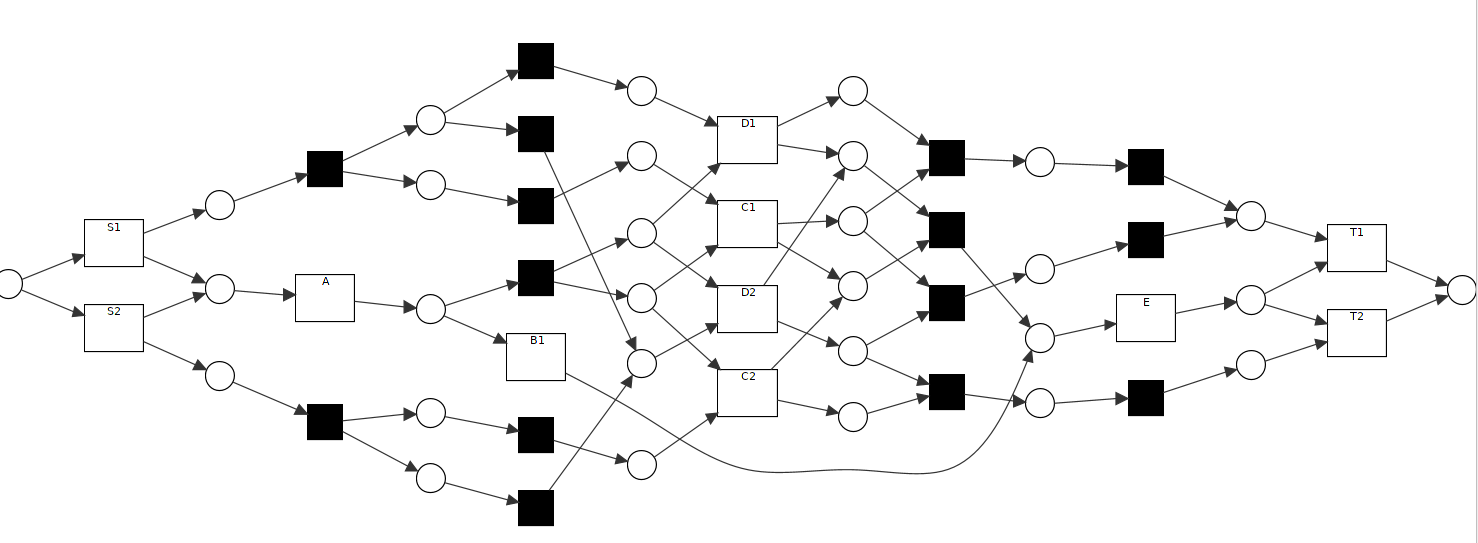
\includegraphics[width=\textwidth]{PN_tc_and_03_01.png}
	\caption{Unsound Repaired Model at Transition B1.}
	\label{fig:unsound_example}
\end{figure}
\fi
\section{Problem Description}
In this section, we use one simple example to deepen our understanding of this problem. 
Given one sound model shown in Fig \ref{fig:seq-2-xor-model} ready for adding long-term dependency on it. 
\begin{figure}[!h]
	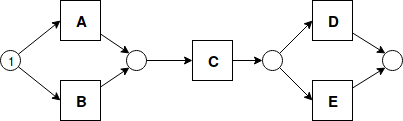
\includegraphics[width=\textwidth]{figures/implementation/LT_Seq_01_Original.png}
	\caption{Simpe Example}
	\label{fig:seq-2-xor-model}
\end{figure}

There are 7 sorts of long-term dependency that is able to happen in this model as listed in the following. Before this, we need to define some concepts at the sake of convenience.
\begin{definition}[Source and Target of Long-term Dependency]
	We define the source set of long-term dependency is  $LT_S:= \{X \vert \exists X, X\rightsquigarrow Y  \in LT \} $, and target set is $LT_T:= \{Y \vert \exists Y, X\rightsquigarrow Y \in LT \} $. \\
	For one xor branch $X \in XORB_S$, the target xor branch set relative to it with long-term dependency is defined as:
	$ LT_T(X)= \{Y \vert \exists Y, X\rightsquigarrow Y \in LT \}$
	Respectively, the source xor branch relative to one xor branch in target is
	$ LT_S(Y)= \{X \vert \exists X, X\rightsquigarrow Y \in LT \}$
\end{definition}
At the same time, we use $XORB_S $ and $XORB_T$ to represent the set of xor branches for source and target xor block. 
\begin{enumerate}
	\item $LT=\{ A\rightsquigarrow D, A\rightsquigarrow E, B\rightsquigarrow D, B\rightsquigarrow D\}$. \\
	$LT_S = \{A,B\}, LT_T=\{D,E\}, \vert LT \vert = \vert XORB_S \vert * \vert XORB_T \vert  $, which means long-term dependency has all combinations of source and target xor branches. 
	\item $LT=\{ A\rightsquigarrow D, A\rightsquigarrow E, B\rightsquigarrow E\}. $\\
	$LT_S = \{A,B\}, LT_T=\{D,E\}$
	$LT_S = XORB_S $ and $LT_T = XORB_T, \vert LT \vert < \vert XORB_S \vert * \vert XORB_T \vert $. it doesn't cover all combinations. But for one xor branch $X \in XORB_S, LT_T(X)= XORB_T$, it has all the full long-term dependency with $XORB_T$. 
	\item $LT=\{ A\rightsquigarrow D, B\rightsquigarrow E\}. $\\
	$LT_S = \{A,B\}, LT_T=\{D,E\}$
	$LT_S = XORB_S $ and $LT_T = XORB_T, \vert LT \vert < \vert XORB_S \vert * \vert XORB_T \vert $. For all xor branch $X \in XORB_S, LT_T(X) \subsetneq XORB_T$, none of xor branch X has long-term dependency with $XORB_T$.
	\item $LT=\{ A\rightsquigarrow D, B\rightsquigarrow D\}.$ \\
	$LT_S = XORB_S ,  LT_T \subsetneq XORB_T$. There exists at least one xor branch $Y \in XORB_T$ which has no long-term dependency on it.
	\item $LT=\{ A\rightsquigarrow D, A\rightsquigarrow E\}.$ \\
	$LT_S \subsetneq XORB_S ,  LT_T = XORB_T$.
	There exists at least one xor branch in source $X \in XORB_S$ which has no long-term dependency on it.
	\item $LT=\{ A\rightsquigarrow E\}. $\\
	$LT_S \subsetneq XORB_S ,  LT_T \subsetneq XORB_T$.
	There exists at least one xor branch in source $X \in XORB_S$  and one xor target xor branch which has no long-term dependency on it.
	\item $ \emptyset$ . There is no long-term dependency on this set. 
\end{enumerate}
For situation 1, it's full connected and xor branches can be chosen freely. So there is no need to add explicit connection on model to represent long-term dependency, therefore the model keeps the same as original. 
For Situation 2 and 3, if $LT_S = XORB_S, LT_T= XORB_T$, then we can create an sound model by adding silent transitions. If not, then we need to use the duplicated transitions to create sound model. But before, we need to prove its soundness. 
For situation 4, 5 and 6, there is no way to prove the soundness even by adding duplicated events. 
For situation 7, I don't think it exists... but if the negative instances has strong effect on it, and make all the connection disappear in long-term dependency but xor branches kept after dfg method??? 
To prove the model sound, we need to prove the four conditions.
\begin{itemize}
	\item safeness. Places cannot hold multiple tokens at the same time
	\item proper completion. If the sink place is marked, all other places are empty.
	\item option to complete. It is always possible to reach the final marking just for the sink place/
	\item no dead part. For any transition there is a path from source to sink place through it. 
\end{itemize}

\section{Discussion of Multiple Implementations}
Until now, multiple methods have been tried to add long-term dependency while trying to keep model sound. Next, we introduce those methods, and give proof if it change its soundness by adding long-term dependency for two xor block in Petri net. 
\subsection{Only Silent Transitions without Duplicated Events}
We add long-term dependency on model by injecting silent transitions and extra places into Petri net. An example is given to describe this method.
\begin{figure}[!h]
	\centering
	\begin{subfigure}[a]{\textwidth}
		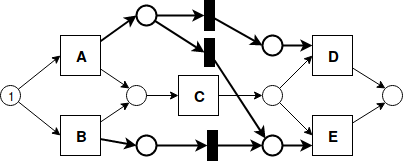
\includegraphics[width=\textwidth]{figures/implementation/LT_Seq_01_Silent_01.png}
		\label{fig:seq-2-silent-1}
		\caption{For situation 2}
	\end{subfigure}
	\hfill
	\begin{subfigure}[b]{\textwidth}
		\centering
		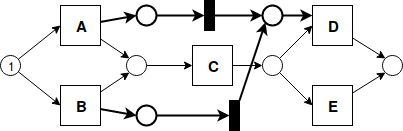
\includegraphics[width=\linewidth]{figures/implementation/LT_Seq_01_Silent_03.png}
		\label{fig:seq-2-silent-2}
		\caption{For situation 4}
	\end{subfigure}
	\hfill
	\begin{subfigure}[c]{\textwidth}
		\centering
		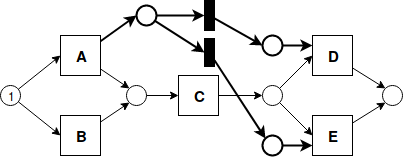
\includegraphics[width=\linewidth]{figures/implementation/LT_Seq_01_Silent_02.png}
		\label{fig:seq-2-silent-3}
		\caption{For situation 5}
	\end{subfigure}
	\label{fig:seq-2-silent-cases}
	\caption{Silent Events for Long-term Dependency}
\end{figure}
This method can not ensure the soundness of model with long-term dependency for situation 4 and 5. \\
\textit{Proof} In Fig \ref{fig:seq-2-silent-2}, it violated the proper completion, and in Fig \ref{fig:seq-2-silent-3}, it can not fire D, E if B is chosen to execute at first. 

\subsection{Full Duplicated Events Without Silent Transitions}
For xor branches which are related to long-term dependency, we duplicate those xor branches in the original xor block, and then connect them together by adding extra place.  An example is given to briefly explain it. 
\begin{figure}[!h]
	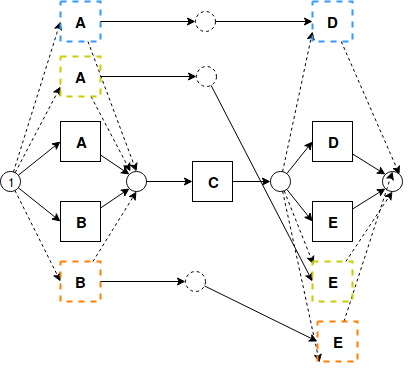
\includegraphics[width=\textwidth]{figures/implementation/LT_Seq_01_FullDuplicated.png}
	\caption{Full Duplicated Events for Long-term Dependency For situation }
	\label{fig:seq-2-full-duplicated}
\end{figure}
In this method, for every item in $LT=\{A\rightsquigarrow D,A\rightsquigarrow E,B\rightsquigarrow D\}$, we duplicate the source and target in corresponding xor block, and then connect the source and target by one explicit place. This method doen not keep the model sound. \\
\textit{Proof:} If original transitions at source xor block are chosen, the execution path is limited to the original transitions in target xor block. It keeps the model sound. If the duplicated transitions at source xor block are chosen (which is colored), two tokens are generated, one for the xor-joint place, one for the extra place. When it comes to target xor block, two kind of transitions are enabled, one is the original transitions, one is the transitions with long-term dependency. But if original transitions are chosen, it violates the proper completion condition for soundness. 

\subsection{Semi Duplicated Events Without Silent Transitions}
This method uses the original transition to express long-term dependency, only adding duplicated events if existing ones are already used for expressing long-term dependency.
\begin{figure}[!h]
	\centering
	\begin{subfigure}[b]{\textwidth}
		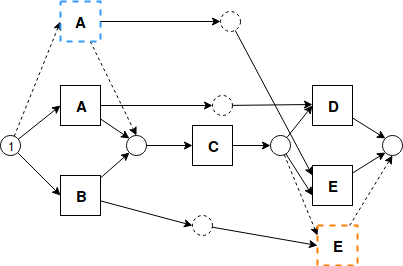
\includegraphics[width=\textwidth]{figures/implementation/LT_Seq_01_SemiDuplicated.png}
		\label{fig:seq-2-semi-duplicated-1}
		\caption{For situation 2}
	\end{subfigure}
	\hfill
	\begin{subfigure}[b]{\textwidth}
		\centering
		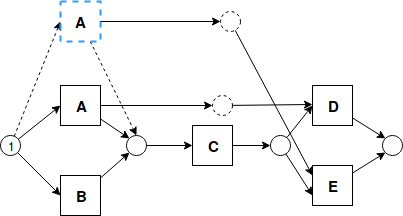
\includegraphics[width=\linewidth]{figures/implementation/LT_Seq_01_SemiDuplicated_Problem2.png}
		\caption{For situation 5}
		\label{fig:seq-2-semi-duplicated-2}
	\end{subfigure}
	\label{fig:seq-2-semi-duplicated-cases}
	\caption{Semi Duplicated Events for Long-term Dependency For situation }
\end{figure}
To express Situation 2 and 3, it create sound model, but for situation 4,5 and 6, it can't guarantee the soundness as shown in the Fig \ref{fig:seq-2-semi-duplicated-2}. Because the transitions in target xor block are not enabled if B is chosen to execute. 

\section{Solution Trials}
To make the generated Petri net sound, there are two thinking ways, one is to make sure that only situation 2 and 3 happen when generating those models. One is to propose a new method to keep it sound. 
In the next subsection, we try to solve this problem by giving constraints to only allow situation 1 2, and 3 available. 
\subsection{Add Constraints}
By adding constraints, we make sure only situations 1,2,3 happen when adding long-term dependency. It requires that after dfg method considers the negative, positive and existing model to delete the unused xor branches for long-term dependency. 
Before doing it, we recover some definitions for long-term dependency detection. 
The definition \ref{def: supported-connection} is rephrased into weight. 
\begin{definition}[Rephrased Correlation of xor branch] The correlation for two branches is expressed into
	\[Wlt(XORB_X,XORB_Y)= Wlt_{ext}(XORB_X, XORB_Y) + Wlt_{pos}(XORB_X, XORB_Y)\] \[ -Wlt_{neg}(XORB_X, XORB_Y)\], where 
	$Wlt_{ext}(XORB_X, XORB_Y)= \frac{1}{|XORB_Y*|}$, $|XORB_{Y*}|$ means the number of possible  directly-follows xor branche set $XORB_{Y*}=\{XORB_{Y1}, XORB_{Y2},...XORB_{Yn} \}$ after $XORB_X$. \\ \\
	$Wlt_{pos}(XORB_X, XORB_Y)= \frac{F_{pos}(XORB_X, XORB_Y)}{F_{pos}(XORB_X, *)}$, \\
	$Wlt_{neg}(XORB_X, XORB_Y)= \frac{F_{neg}(XORB_X, XORB_Y)}{F_{neg}(XORB_X, *)}$, \\	
\end{definition}
The $F_{pos}(XORB_X, XORB_Y)$ and $F_{neg}(XORB_X, XORB_Y)$ are the frequency of the coexistence of $XORB_X$ and $XORB_Y$, respectively in positive and negative event log.

With this rephrased definition, to make the model sound, we need to prove, if there is a xor branch $XORB_Y$ in the generated process tree, there must exist one long-term dependency related to it, $\exists XORB_X, Wlt(XORB_X,XORB_Y) >$ lt-threshold. We formalize this problem. Else, the model can't be sound!!
\begin{proposition}
	Given a process tree, a pair of xor branch set, $(B_A,B_B)$ with $B_A={XORB_{X1}, XORB_{X2},...XORB_{Xm}}, B_B={XORB_{Y1}, XORB_{Y2},...XORB_{Yn}}$, the obligatory part between $B_A$ and $B_B$ is marked M, it is to prove:: \\
	$\forall XORB_Y \in B_B$, if $W(M, XORB_Yj) > threshold$, \\ then there exists one $XORB_Xi \in B_A$ with 
	\[Wlt(XORB_Xi, XORB_Yj)> \text{lt-threshold}\]. 
\end{proposition}
Given a simplified scenes, it is listed in Fig \ref{fig:simplified-graph-model}. M is an obligatory path from the set $\{X1,X2,..Xm\}$ to $\{Y1,Y2,..Yn\}$. If there exists directly-follows relation of M and Y1, then there must exist one long-term dependency of Xi and Y1. 

\begin{figure}[!h]
	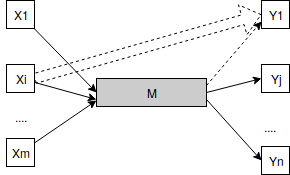
\includegraphics[width=\textwidth]{figures/implementation/RelationOfThreshold-LTThreshold.png}
	\caption{Simplified Graph MOdel}
	\label{fig:simplified-graph-model}
\end{figure}

The definition of $W(M, XORB_{Yj})$ is reviewed below.
\begin{definition}[Assign new weights to graph $G_{new}$]
	there are three weights from $G_{pos}$, $G_{neg}$ and $G_{ext}$, the new weight is 
	\begin{itemize}
		\item For one directly-follows relation, \[ W(E_{G_{new}}(A,B)) = Weight(E_{G_{pos}}(A,B)) + Weight(E_{G_{ext}}(A,B)) - Weight(E_{G_{neg}}(A,B))\]
		\item Given a directly-follows graph G(L), the weight of each directly-follows relation is defined as \[ Weight(E(A,B)) = \frac{Cardinality(E(A,B))}{Cardinality(E(A,*))}  \] 
	\end{itemize}
\end{definition}

When prove by contradiction, we assume that the opposite proposition is true. If it shows that such an assumption leads to a contradiction, then the original proposition is valid. 
\begin{proposition}
	for one xor branch $XORB_Y$, if $W(M, XORB_{Yj}) > threshold$, \\ there exists no one $XORB_{Xi}$ with 
	\[Wlt(XORB_{Xi}, XORB_{Yj})<\text{lt-threshold}\]. 
\end{proposition}

Or we change to another thinking way to get the relation of threshold and lt-threshold, such that we have the theorem valid. Then we rephrase the question into
\begin{proposition}[Another way of thinking]
	Given a process tree, a pair of xor branch set, $(B_A,B_B)$ with $B_A=\{XORB_{X1}, XORB_{X2},...XORB_{Xm}\}, B_B=\{XORB_{Y1}, XORB_{Y2},...XORB_{Yn}\}$, the obligatory part between $B_A$ and $B_B$ is marked M. If,\\
	for one xor branch $XORB_{Yj}$, if $W(M, XORB_{Yj}) > threshold$, \\ there exists one $XORB_Xi$ with 
	\[Wlt(XORB_{Xi}, XORB_{Yj})> \text{lt-threshold}\]
	What is the relation of threshold and lt-threshold?? 
\end{proposition}
If we expand the theorem, we need to prove 
\begin{proposition}[Relation of threshold and lt-threshold]
	What is the relation of threshold and lt-threshold, to make the following proposition valid. If 
	\begin{equation*}
	\begin{gathered}
	W(M, XORB_{Yj})  > threshold \\
	W(M, XORB_{Yj}) = Weight(E_{G_{pos}}(M, XORB_{Yj})) \\
	+ Weight(E_{G_{ext}}(M, XORB_{Yj})) 
	- Weight(E_{G_{neg}}(M, XORB_{Yj})) \\
	\frac{1}{|Y*|} + \frac{\sum_{Xi}{Cardinality(M,Yj|Xi)}} {\sum_{Xi}{Cardinality(M,Y*|Xi)}}  
	- \frac{\sum_{Xi}{Cardinality(M,Yj|Xi)\prime}} {\sum_{Xi}{Cardinality(M,Y*|Xi)\prime} > threshold} \\
	\text{Then, exist one Yj with}\\
	Wlt(Xi, Yj)> \text{lt-threshold} \\
	Wlt{ext}(Xi, Yj) + Wlt{pos}(Xi, Yj) -Wlt{neg}(Xi, Yj) > \text{lt-threshold}\\
	\frac{1}{|Y*|} + \frac{Cardinality(M,Yj|Xi)} {Cardinality(M,Y*|Xi)}  
	- \frac{Cardinality(M,Yj|Xi)\prime} {Cardinality(M,Y*|Xi)\prime} > \text{lt-threshold}  \\
	\text{Or \textbf{there is a contradiction when all Yj}}\\
	Wlt(Xi, Yj)< \text{lt-threshold}\\
	\sum_{Xi} Wlt(Xi, Yj) < |X*|\bullet \text{lt-threshold} \\
	\frac{|X*|}{|Y*|} + \sum_{Xi}\frac{Cardinality(M,Yj|Xi)} {Cardinality(M,Y*|Xi)}  
	- \sum_{Xi}\frac{Cardinality(M,Yj|Xi)\prime} {Cardinality(M,Y*|Xi)\prime} < |X*|\bullet \text{lt-threshold}  \\
	\end{gathered}
	\end{equation*}	
	$Cardinality(M,Yj|Xi)$ means the frequency of coexistence of M and Yj given Xi in the trace in positive, while $Cardinality(M,Yj|Xi)\prime$ represents the frequency in negative. $Cardinality(M,Y*|Xi)$ is the sum frequency of set ${Y1,..Yj,..Yn}$, it equals to \[Cardinality(M,Y*|Xi) = \sum_{Yi}Cardinality(M,Yj|Xi)\]
\end{proposition}
If we set them into zero, there is a lot of existing edges kept into the old method with no evidence in event log to support the connection. 

\subsection{New Method Proposal}
we can add silent transition to make the model sound??? To combine the duplicated events and silent transitions. But how is it and how to prove its soundness?? 

The problem is around situation 4 ,5 and 6. If we have the negative evidence to avoid the long-term dependency. 
For situation 4, $LT=\{ A\rightsquigarrow D, B\rightsquigarrow D\}$. It shows in those two situations. 
\begin{itemize}
	\item If E is kept due to the existing model, and no positive and negative evidence is given for long-term dependency, then Wlt is positive to add long-term dependency on it. 
	\item If long-term dependency is prohibited due to the negative instances, so we need to delete the execution of E by substituting it by silent transitions, and then deleted from the model. Further, after deleting those events, we check the long-term dependency again. If it have full long-term dependency combination, no need to explicitly address them in the model. Else, the explicit long-term dependency is kept in the model. 
\end{itemize}
We can solve it by adding silent transitions in the xor blocks to represent the long-tem dependency. 
\begin{figure}[!h]
	\centering
	\begin{subfigure}[b]{\textwidth}
		\centering
		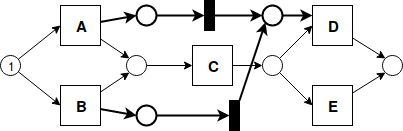
\includegraphics[width=\linewidth]{figures/implementation/LT_Seq_01_Silent_03.png}
		\label{fig:seq-2-silent-2-original}
		\caption{For situation 4}
	\end{subfigure}
	\hfill
	\begin{subfigure}[b]{\textwidth}
		\centering
		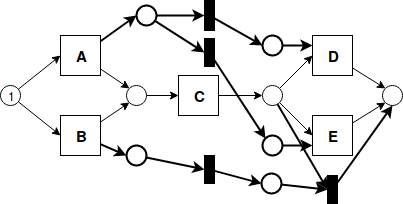
\includegraphics[width=\linewidth]{figures/implementation/LT_Seq_01_Silent_03_AfterAddition.png}
		\label{fig:seq-2-silent-afteraddition}
		\caption{For situation 4}
	\end{subfigure}
	\hfill
	\begin{subfigure}[c]{\textwidth}
		\centering
		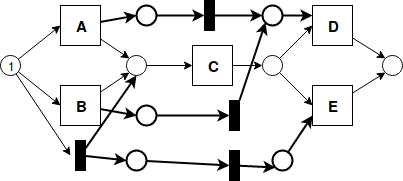
\includegraphics[width=\linewidth]{figures/implementation/LT_Seq_01_Silent_02_AfterAddition.png}
		\label{fig:seq-2-silent-afteraddition-2}
		\caption{For situation 5}
	\end{subfigure}
	\label{fig:seq-2-silent-changes}
	\caption{Silent Events for Long-term Dependency}
\end{figure}

\iffalse
In this way, the final generated models with respect to Fig \ref{fig:seq-2-silent-2} and \ref{fig:seq-2-silent-3} are changed to sound model. 
\begin{figure}[!h]
	\centering
	\begin{subfigure}[b]{\textwidth}
		\centering
		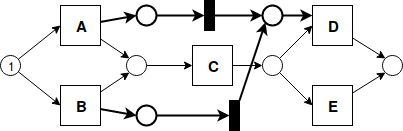
\includegraphics[width=\linewidth]{figures/implementation/LT_Seq_01_Silent_03.png}
		\label{fig:seq-2-silent-2-original}
		\caption{For situation 4}
	\end{subfigure}
	\hfill
	\begin{subfigure}[b]{\textwidth}
		\centering
		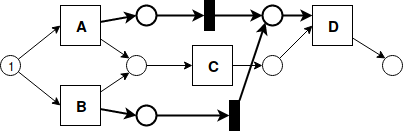
\includegraphics[width=\linewidth]{figures/implementation/LT_Seq_01_Silent_03_AfterDeletion.png}
		\label{fig:seq-2-silent-afterdeletion}
		\caption{For situation 4}
	\end{subfigure}
	\hfill
	\begin{subfigure}[c]{\textwidth}
		\centering
		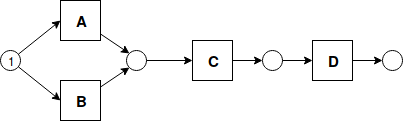
\includegraphics[width=\linewidth]{figures/implementation/LT_Seq_01_Silent_03_AfterDeletion_02.png}
		\label{fig:seq-2-silent-afterdeletion-2}
		\caption{For situation 5}
	\end{subfigure}
	\label{fig:seq-2-silent-changes}
	\caption{Silent Events for Long-term Dependency}
\end{figure}
The similar procedure is done in situation 5, the event B is deleted from the original model, which results in Fig \ref{fig:seq-2-silent-5}.  For situation 6, we combine the procedure for situation 4 and 5, and get the model in Fig \ref{fig:seq-2-silent-6}.
\begin{figure}
	\centering
	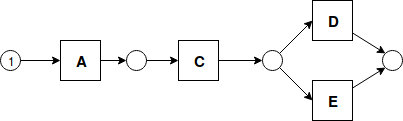
\includegraphics{images/LT_Seq_01_Silent_02_AfterDeletion.png}
	\caption{Caption}
	\label{fig:seq-2-silent-5}
\end{figure}
\begin{figure}
	\centering
	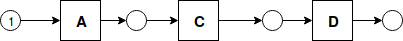
\includegraphics{figures/implementation/LT_Seq_01_Silent_04_AfterDeletion.png}
	\caption{Caption}
	\label{fig:seq-2-silent-6}
\end{figure}
We need to prove the cutting makes the model sound!! By deleting the unused events in target xor block, token passes through another exclusive xor branches. 
Is there any cases that it affects another xor block?? The answer is Yes, if those block is used as source xor block, and it leads to positive long-term dependency, then we need to keep it here!! Deletion causes trouble, too!!  
\fi

More details here are around 6 pages